\section{Experimental Procedure\label{sec:VT-experimentalProcedure}}

The observed time-averaged spatial off-set of the particles inside the optical 
trap is naturally zero, but the frequency content of the observed particle 
motion includes the thermal energy content of the particle as well as its 
rotational frequency. The angular frequency appears as an additional peak in the 
power spectrum of the rotating particle. In order to validate this detection 
method, particles with a rotational rate of less than \SI{1.66}{\hertz} 
(\SI{100}{\rpm}) were observed by a high-speed camera (HiSpec1 G2 Mono, Fastec, 
San Diego, USA) while also recording their power spectrum.  In the validation 
experiments the transparent device was filled with \SI{4.39}{\micro\meter} 
silica glass micro-spheres suspended in distilled water at a low concentration 
of a few particles per \si{\micro\liter}.  This low particle concentration does 
not effect the ratio $\tilde{\rho} = \sfrac{\rho_{\text{s}}}{\rho_{\text{f}}}$. 
The open channel ends were sealed with silicone oil to ensure a constant fluid 
volume during the measurements.

\subsection{Rotation Detection 
Validation\label{sec:VT-rotationDetectionValidation}}

Two sets of validation experiments were performed: (i) non-spherical particle 
rotation with slightly non-spherical particles; (ii) spherical particle rotation 
with gold covered particles for increased contrast in the video observation 
\cite{Lamprecht}. 

According to \citeauthor{hahn2016} \cite{hahn2016}, non-spherical objects can 
also be rotated due to the acoustic VT, but here effects of acoustic radiation 
torques may govern or influence their rotations \cite{wang2012time}. A slightly 
non-spherical \SI{4.39}{\micro\meter} silica particle (see \cref{fig:Fig5}) was 
trapped in the optical potential well with \SI{100}{\milli\watt} laser power and 
moved to the reference position ($x,y,z = 0$) in the center of all three 
dimensions of the fluid chamber. The acoustic pressure field is formed by two 
orthogonal standing waves at the same excitation frequency of 
\SI{1090}{\kilo\hertz} and \SI{10.0}{\Vrms} amplitude. The particle was then 
optically moved to the closest resulting pressure node (intersection of two 
pressure nodal lines in $x$- and $y$-direction) with respect to the reference 
position. Positions of the pressure nodes were determined by a previous set of 
experiments.

The phase difference between the acoustic excitation directions $x$- and 
$y$-direction was set to $\zeta=\sfrac{\pi}{2}$, and the non-spherical particle 
rotated counter-clockwise with $\Omega = \SI{1.12}{\hertz}\,(\SI{67}{\rpm})$ 
(arithmetic mean of \SI{0.3}{\hertz} (\SI{18}{\rpm}) and \SI{1.6}{\hertz} 
(\SI{96}{\rpm}); see also \cref{fig:Fig5}). At $\zeta=0$ the particle did not 
rotate because of the stable, non-varying acoustic potential.

%%%%%%%%%%%%%%%%%%%
\begin{figure}
    \centering
    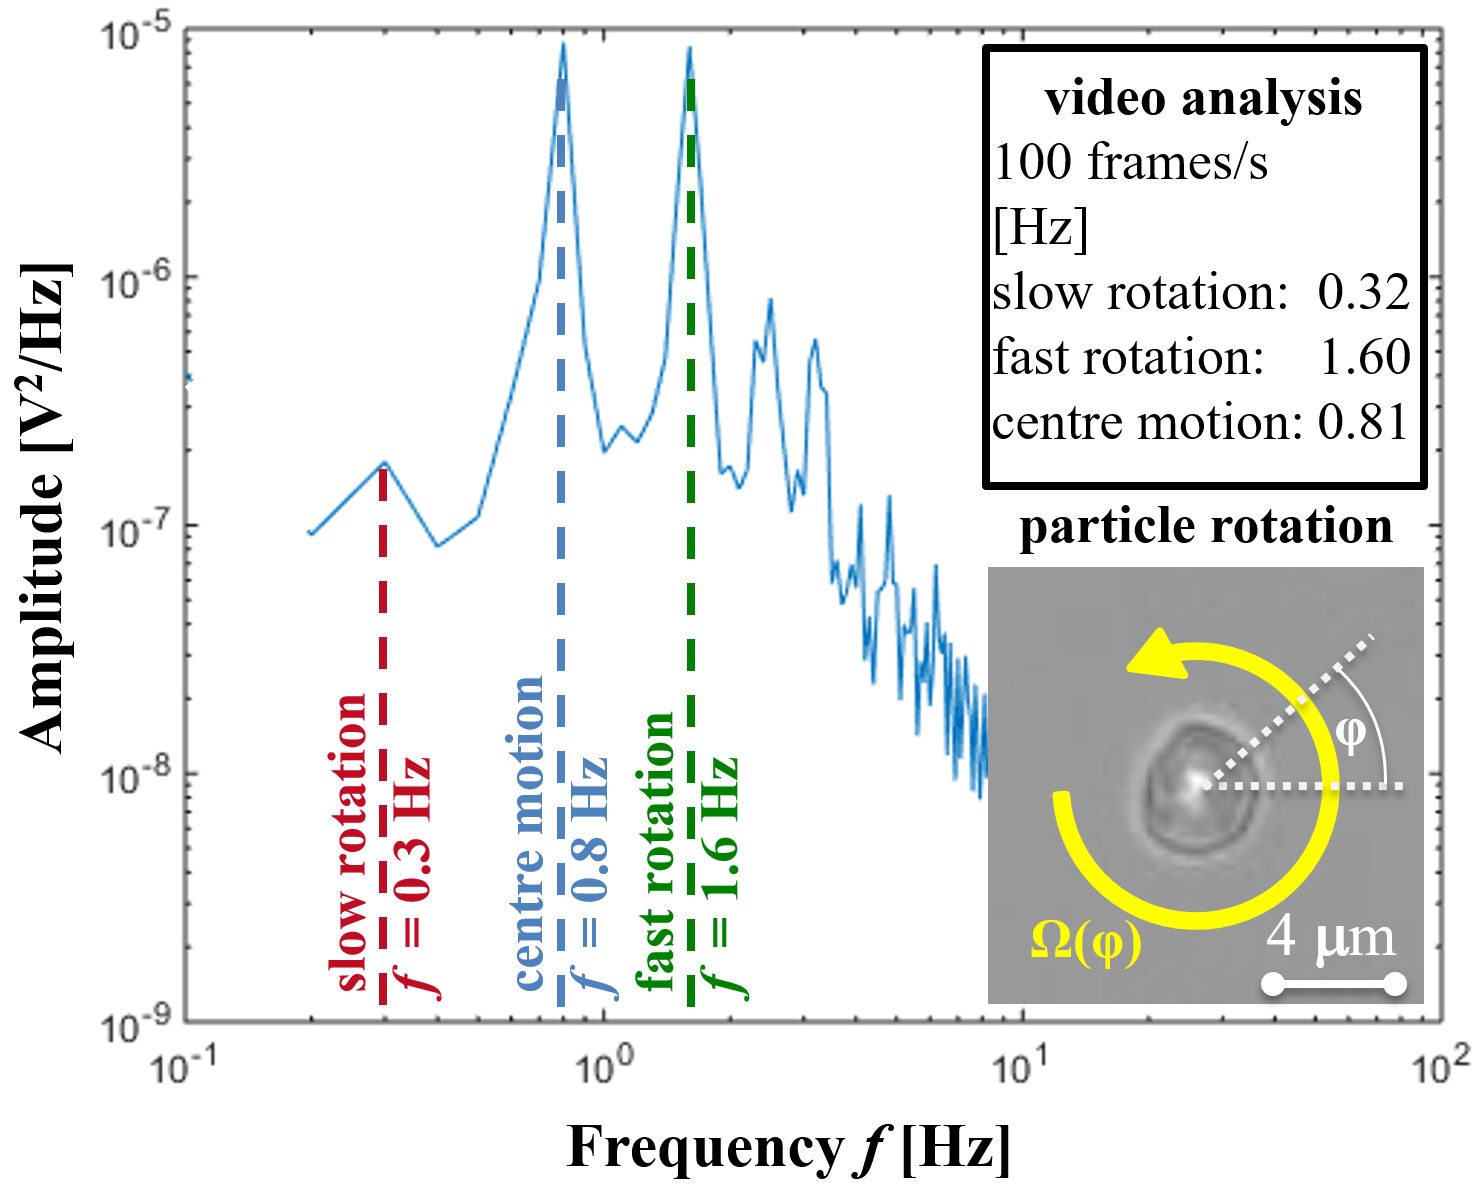
\includegraphics[width=84mm]{Fig5.png}
    \caption{Power spectral density and results of the video analysis of a 
      counter-clockwise rotating non-spherical silica particle at 
      \SI{1090}{\kilo\hertz} and \SI{10.0}{\Vrms} with relative phase shift of 
      $\zeta= \sfrac{\pi}{2}$. The 10 times averaged power spectrum of the 
      $y$-signal of the detection unit (QPD) was recorded with a frequency 
      resolution of $\Delta f = \SI{0.1}{\hertz}$ and a sampling rate of 
      \SI{1}{\MS}. Three main peaks were observed at \numlist{0.3; 0.8; 1.6} 
      \si{\hertz}. The frequency peak at \SI{0.8}{\hertz} corresponds to a 
      relative $xy$-motion of the trapped particle, whereas the peaks at 
      \numlist{0.3; 1.6} \si{\hertz} (\numlist{18;96} \si{\rpm}) are related to 
      a non-constant angular rotation $\Omega(\varphi)$ of the particle. The 
      measured results are in correlation with the determined rotational rate by 
      the high-speed video analysis with a frame rate of \SI{100}{\fps}. See the 
      supplemental material for a optically trapped particle rotating 
      sequentially with two velocities due to its imperfect spherical 
  shape.\label{fig:Fig5}}
\end{figure}%
%%%%%%%%%%%%%%%%%%%

In \cref{fig:Fig5}, the average of 10 power spectral density plots is depicted, 
each obtained from a \SI{10}{\second} recording. The frequency resolution is 
$\Delta f=\SI{0.1}{\hertz}$. Three main peaks were observed in the power 
spectrum at \numlist{0.3; 0.8; 1.6} \si{\hertz}, which correlate with the 
frequencies detected by the contemporaneous video detection. We see these peaks 
on both QPDs for the $x-$ and $y$-direction. However for some of the latter 
rotational measurements, the $xy$-motion of the particle adds more peaks 
depending on the major axis of the acoustic displacement. All other peaks are 
related to multiple repetitions of these angular frequencies due to deviations 
of the spherical shape of the particle.  The peak at \SI{0.8}{\hertz} 
corresponds to a relative $xy$-motion of the particle, whereas the peaks at 
\numlist{0.3; 1.6} \si{\hertz} are related to angular frequencies of the 
non-constant rotation $\Omega(\varphi)$ of the particle. The existence of two 
frequency peaks is related to the influence of different acoustic pressures in 
$x$ and $y$-direction because the amplitude were not yet matched for this 
validation.  Hence, the acoustic radiation forces on the particle have different 
magnitudes in $x$ and $y$-direction. So, the distribution of acoustic radiation 
pressure on the particle changes during its rotation and leads to an additional 
orientation dependent acoustic radiation torque.  The influence of acoustic 
radiation forces on particle orientations is a well-known effect for small 
non-spherical particles with $r \ll \lambda$ \cite{konig1891,garbin2015}, but 
this experiment shows that this influence is also large enough to influence the 
rotation by the acoustic VT.  Particles with a larger degree of 
non-sphericalness did not even start to rotate in this set of experiments. This 
is in agreement with the predictions of \citeauthor{hahn2016} \cite{hahn2016}, 
that the acoustic VT decreases with a higher degree of elliptical shape of the 
particles. In contrast, the acoustic radiation torque increases and hinders a 
constant rotation of the particle, if the symmetry of the experimental acoustic 
potential at $\zeta= \sfrac{\pi}{2}$ is imperfect.

Previously, optical traps formed by a linearly polarized laser have been applied 
to rotate anisotropic particles \cite{GutirezMedina2010}. However, this torque 
is dependent on the orientation of the anisotropic particle with respect to the 
polarization plane of the laser. If the laser power is high enough, the 
acoustically induced rotation can be inhibited because the anisotropic particle 
is optically locked to the polarization plane. For perfectly spherical particles 
without any shape anisotropy this optical torque vanishes 
\cite{Manzo2006,Friese1998}. We did not observe influences of optical forces on 
the final rotational velocities of the spherical particles because the 
determined velocities in the experiments were independent of the applied laser 
power. For our validation experiments with deformed and gold coated particles we 
did not investigate further the influence of the linearly polarized laser on the 
particles. This indicates that the applied acoustic torque was greater in 
magnitude than the optical torque.

Also, the experiments that are presented afterward show that the particle 
rotation is dominated by the acoustic field. By moving the particle through the 
flow cell or by changing the phase of the excitation signal, the rotation can be 
stopped, started and reversed (see \cref{fig:Fig8} and the video in the 
supplemental material).

A closer investigation was not possible in our current experimental set-up 
because particles sank due to gravity if the laser was turned off. Observed 
rotations near fluid boundaries (bottom plate) are governed by influences of 
near-boundary effects, e.g.\ higher viscous drag, different acoustic scattering 
and streaming which would complicate an investigation of low laser powers on the 
particle rotation.

The second set of validation experiments employed spherical particles with a 
thin gold layer to increase the contrast for the video observation 
\cite{Lamprecht}. The additional gold layer changed the optical properties of 
the particles and led to a different optical trapping behavior in the 
experiments. Most of the particles could not be trapped optically because the 
gold layer reflected the incident laser light (\SI{785}{\nano\meter}) and the 
resulting optical scattering forces pushed the particles away from the laser 
focus \cite{Mousavi2019,ashkin1992,Svoboda}. The particle needs to be 
transparent for the wavelength of the laser, in order to enable trapping. 
However, due to statistical variations of the coating process some particles 
were optically trappable, since just a small portion of the surface was coated.  
And hence, just a small portion of the incoming laser was reflected. One example 
of an optically trapped particle with a constant and stable rotation is shown in 
\cref{fig:Fig6}. The brighter regions at the surface of the particle arise from 
the reflected laser light due to the partial gold coating.  These regions 
rotated with the optically trapped particle due to the acoustic VT.\@ The 
angular change of reflected light on the particle surface was then determined by 
the QPDs of the optical detection unit and increased the signal strength by a 
factor of 100 with respect to uncoated particles. The recorded power spectrum of 
the $x$- and $y$-signals included the information about the angular frequency of 
the rotating particle.

An example for a recorded power spectrum of a rotating gold-layered 
\SI{4.39}{\micro\meter} silica particle at an acoustic excitation frequency of 
\SI{1090}{\kilo\hertz} and amplitude of \SI{2.5}{\Vrms} with a relative phase 
shift of $\zeta= \sfrac{\pi}{2}$ is depicted in \cref{fig:Fig6}. A clear peak 
can be seen at \SI{1.3}{\hertz}. The determined rotational rate of the particle 
by video observations was \SI{1.31}{\hertz} (\SI{78.6}{\rpm}), which correlates 
with the measured peak at \SI{1.3}{\hertz} (\SI{78.0}{\rpm}).  A further 
variation of the acoustic excitation parameters (amplitude and relative phase) 
shifted the peaks in frequency as predicted by \cref{eq:VT-Eq1,eq:AcGovEqConti} 
(results are not shown) \cite{Lamprecht}.

%%%%%%%%%%%%%%%%%%%
\begin{figure}
    \centering
    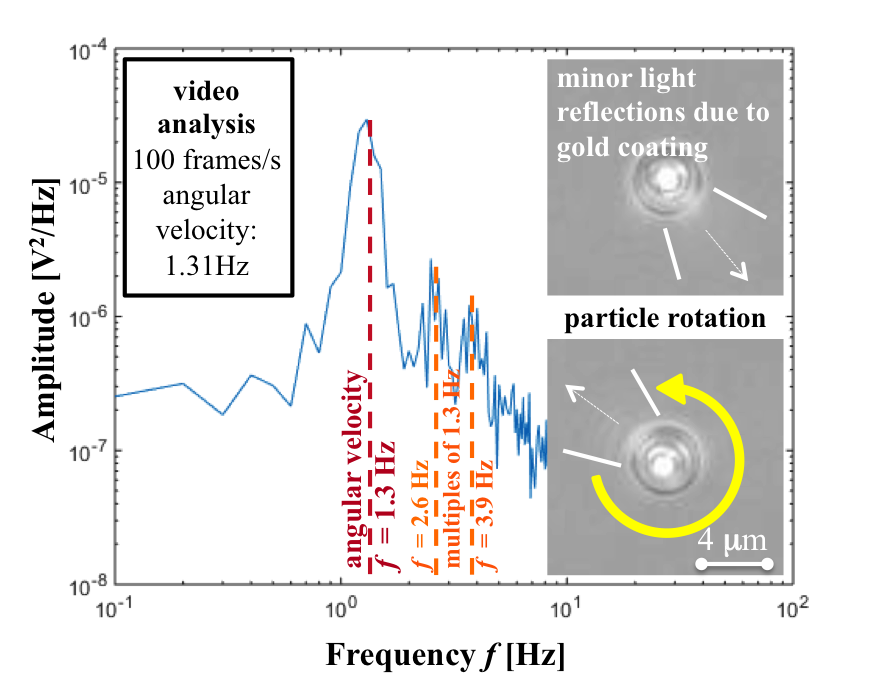
\includegraphics[width=84mm]{Fig6.png}
    \caption{Power spectral density and results of the video analysis of a 
      counter-clockwise rotating gold-coated spherical \SI{4.39}{\micro\meter} 
      silica particle at \SI{1090}{\kilo\hertz} and \SI{2.5}{\Vrms} with 
      relative phase shift $\zeta= \sfrac{\pi}{2}$. The 10 times averaged power 
      spectrum of the $y$-signal of the detection unit (QPD) was recorded with a 
      frequency resolution of $\Delta f=\SI{0.1}{\hertz}$ and a sampling rate of 
      \SI{1}{\MS}. A clear peak at \SI{1.3}{\hertz} and two additional peaks at 
      \numlist{2.6; 3.9} \si{\hertz} were observed. The amplitudes of the 
      additional peaks were one order of magnitude smaller as the amplitude of 
      the peak at \SI{1.3}{\hertz}. The peak at \SI{1.3}{\hertz} correlates with 
  the determined rotational rate by the high-speed video analysis at a frame 
  rate of \SI{100}{\fps}.\label{fig:Fig6}}
\end{figure}%
%%%%%%%%%%%%%%%%%%%

\subsection{Rotation of particles where $\normBdLayer \approx 
1$\label{sec:VT-rotationParticles}}

The determinations of the rotational rate with the power spectrum-method opened 
the possibility to measure fast rotations ($>\SI{25}{\hertz}$ (\SI{1500}{\rpm})) 
of particles with a radius $R$ about \SI{1}{\micro\meter}.  For such small 
particles the ratio of the thickness of the viscous boundary layer $\delta$ and 
the particle radius $R$ approaches 1 ($\normBdLayer \approx 1$) in the 
\si{\mega\hertz}-range (\SIrange{1}{10}{\mega\hertz}). The analytical formulas 
become invalid for the case that $\normBdLayer > \sfrac{1}{15}$ \cite{hahn2016}.  
Particle rotations within the limit $\normBdLayer \approx 1$ were experimentally 
validated by an investigation of silica spheres with a \SI{2.06}{\micro\meter} 
(Microparticles GmbH, Berlin, Germany) diameter resuspended with a 
water/glycerol (70$\%$/30$\%$) mixture.  The viscosity $\mu_f$ of the aqueous 
glycerol solution was \SI{0.06}{\pascal\second} \cite{jerome1968} with a 
determined density of \SI{1.1}{\gram\per\centi\meter\cubed} (dense knife, DMA 
35N, Anton Paar GmbH, Graz, Austria) and increased the thickness of the viscous 
boundary layer to approximately \SI{1.33}{\micro\meter} at an excitation 
frequency of \SI{1043}{\kilo\hertz} ($\lambda \approx \SI{1.4}{\mm}$). The 
normalized viscous boundary layer is therefore $\normBdLayer \approx 1.30$.

The optical trapping set-up was originally designed to measure the acoustic 
force and pressure amplitudes inside micro-fluidic channels and cavities 
\cite{Lakamper,Lamprecht2016}. The same procedure was used here to measure the 
local acoustic pressure amplitudes inside the fluid chamber of the transparent 
micro-device. An accurate prediction of the acoustic pressure amplitudes $A_{X}$ 
and $A_{Y}$ of the two orthogonal standing waves was important to determine the 
strength of the acoustic VT by observing the steady-state rotational rate 
$\finalOmega$ of rotating particles.

Therefore, the local acoustic pressure amplitudes $A_{X}$ and $A_{Y}$ were 
individually measured in $x$- and $y$-direction by exciting only one transducer 
of the corresponding $x$- or $y$-direction, respectively. We measured the 
acoustic forces in all three dimensions ($x$, $y$, $z$) acting on the 
\SI{2.06}{\micro\meter}-particle inside the optical trapping potential. The 
spatial measurement range was $\pm \SI{0.55}{mm}$ in the $x$- and $y$-direction.  
The point $(\SI{0.21}{\mm}, \SI{0.22}{\mm})$, measured relatively to the middle 
of the fluid chamber, corresponded to the spatial position where a pressure 
nodal line in $x$- and $y$-direction overlapped.

The maximal force amplitudes at \SI{1043}{\kilo\hertz} were 
\SIrange{-96}{+25}{\femto\newton} for the $x$-direction and 
\SIrange{-32}{28}{\femto\newton} for the $y$-direction. The peak-to-peak value 
of the determined forces in $y$-direction was about two times weaker than in 
$x$-direction. This factor of 2 was used to calibrate the piezoelectric 
excitation amplitude to reach equal acoustic pressure amplitudes in both 
excitation directions.

The excitation amplitude $U_{el}$ is proportional with the acoustic pressure 
amplitude $A_{x,y}$ ($U_{el} \propto A_{x,y}$), whereas the acoustic radiation 
force $F_{ac}$ has a quadratic dependency of the acoustic pressure amplitudes 
$A_{x,y}$ ($F_{ac} \propto A_{x,y}^2$) \cite{Barnkob2}. Therefore, the 
excitation amplitude of the piezoelectric transducer in $y$-direction was 
increased by a factor of $\sqrt{2}$ for all further investigations. The acoustic 
pressure amplitude $p_{a}$ was calculated via
%%%%%%%%%%%%%%%%%%%
\begin{equation}
\label{eq:VT-PressurePredictions}
p_{a}^{2} = \frac{F}{\pi\,R^{3}\,\kappa_{0}\,\Phi(f_{1},f_{2})} 
\frac{1}{k\,\sin(2k\,x)} =
\frac{F}{\pi\,R^{3}\,\kappa_{0}\,\Phi(f_{1},f_{2})} 
\frac{\lambda_{\text{p}}}{2\pi\,\sin(x\,\sfrac{4\pi}{\lambda_{\text{p}}})}
\end{equation}
%%%%%%%%%%%%%%%%%%%
where a 1-dimensional standing plane wave is assumed \cite{Bruus2012}. $F$ is 
the force measured with the optical trap, $\lambda_{\text{p}}$ the wavelength of 
the pressure field, $k = \sfrac{2\pi}{\lambda_{\text{p}}}$ the wavenumber, $R$ 
the radius of the spherical particle, $\kappa_{0}$ the compressibility of the 
fluid, $\Phi(f_{1},f_{2})$ the so-called acoustic contrast factor, and 
$\sin(kx)$ the spatial dependency of the standing wave.  Since the force was 
measured at the force maximum $\sin(2\,kx)$ is set to $\sin(\sfrac{\pi}{2}) = 
1$. In addition, because of the value for the normalized viscous boundary layer 
$\normBdLayer \approx 1$, the corrected dipole factor  
$f_{2}(\tilde{\rho},\normBdLayer)$ of \citeauthor{Settnes2012} 
\cite{Settnes2012} was utilized. With this, the determined acoustic pressure 
amplitude for the standing wave in $x$-direction was \SI{245}{\kilo\pascal} for 
the measured acoustic forces and wavelength if an influence of acoustic 
streaming was neglected. 

After the calibration of the excitation amplitudes and the acoustic pressures of 
both acoustofluidic channels the acoustic VT was quantitatively investigated 
inside the fluid chamber. One \SI{2.06}{\micro\meter} silica particle was 
optically trapped and moved in $x$-direction inside the wave field of two 
orthogonal standing waves, while measuring its power spectrum at specified 
measurements points. The location of one specific pressure nodal line for an one 
dimensional standing wave in $x$- and $y$-direction at \SI{1043}{\kilo\hertz} 
was determined at $x=\SI{0.21}{\mm}$ and $y=\SI{0.22}{\mm}$, respectively. These 
nodal lines formed a local pressure node at their intersection if the acoustic 
excitation was shifted in phase with $\zeta = \sfrac{\pi}{2}$. There, the 
acoustic VT had its maximum value. Therefore, a measurement line in 
$x$-direction was defined between $x=0.20\pm0.55~\si{\milli\meter}$ at constant 
$y=\SI{0.22}{\milli\meter}$.

The particle exerted a counter-clockwise rotation at the local pressure node due 
to the acoustic VT at \SI{1043}{\kilo\hertz} with \SI{10.0}{\Vrms} and 
\SI{14.2}{\Vrms} excitation amplitude in $x$- and $y$-direction, respectively.

The detection of the angular frequency in a recorded power spectrum was not 
trivial for those small and spherical silica particles due to their low 
signal-to-noise ratios. Additionally, the power spectrum was disturbed by added 
frequencies of the acoustic excitation set-up; namely, an additional peak at 
\SI{100}{\hertz} originating from the voltage supply and \SI{170}{\hertz} from 
the amplifier itself.  Therefore, all measurements were repeated with a 
ten-times lower excitation amplitudes in $x$- and $y$-direction to calibrate the 
power spectrum measurements due to unknown influences of the environment and 
attached set-ups. An initialization of particle rotations was not observed at 
these low excitation amplitudes. A peak detection algorithm (implemented in 
MatLab) used the calibration measurement to eliminate disturbances on the 
determined power spectrum of a locally rotating particle due to VT.\@

\Cref{fig:Fig8} depicts the power spectrum of a rotating particle with a clear 
peak at a frequency of \SI{165}{\hertz}. The particle was located at the 
relative location (-0.075, 0.220) \si{\mm} and its rotation was initialized at 
\SI{1043}{\kilo\hertz} with an excitation amplitude of \SI{10.0}{\Vrms} and 
\SI{14.2}{\Vrms} in $x$- and $y$-direction, respectively.  An appearance of 
additional peaks at a multiple of the angular frequency was not monitored by the 
peak-detection algorithm, likely because the amplitude of these peaks was below 
the noise floor. Their signal strength was expected to be one order of magnitude 
smaller (see \cref{fig:Fig5,fig:Fig6}).  The detection algorithm had a threshold 
value of 3 (signal-to-noise ratio) for indicating peaks in determined power 
spectrum.  \cref{fig:Fig8}b depicts the corresponding calibration power spectrum 
of \cref{fig:Fig8}a.

\Cref{fig:Fig10} depicts the peaks detected by the peak-detection algorithm. 
Each point represents a separate rotational rate measurement. Interestingly, the 
strength of the angular frequency peaks was proportional to Brownian noise with 
$\sfrac{1}{f^2}$. These peaks are due to the particle rotations at positions 
within the spatial range of $x=0.21\pm\SI{0.55}{\mm}$ and $y=\SI{0.22}{\mm}$.  
The spatial dependency and formation of these peaks were in correlation with 
\cref{eq:VT-Eq1} and the maximal frequency $f$ of a peak in the power spectrum was 
\SI{229}{\hertz} ($ \finalOmega = \SI{13.8e3}{\rpm} $). The quantitative 
analysis revealed that maximal rotation appeared at $x=\SI{0.16}{\mm}$ (pressure 
node) and the resulting acoustic wavelength in $x$-direction was \SI{1.9}{\mm}.  
A one-dimensional wave in water at $f=\SI{1043}{\kilo\hertz}$ predicts an 
acoustic wavelength of $\lambda = \sfrac{c}{f} \approx \SI{1.4}{\mm}$ (compare 
\cref{fig:Fig4}). The difference in wavelength from \cref{fig:Fig4} ($\lambda 
\approx \SI{1.4}{\mm} $) to the fitted value of $\lambda \approx \SI{1.9}{\mm} $ 
may be related to an off-set in orientation of the 3-dimensional wavenumber 
$|\bm{k}|^{2} = k^{2}_{x} + k^{2}_{y} + k^{2}_{z}$ in the optical trapping 
set-up. Eigenfrequencies and their acoustic fields are influenced by the 
optical trapping set-up due to the additional interface between the 
acoustofluidic device and the water-immersion objective \cite{Lamprecht2016}.  
\Cref{fig:Fig4} was observed with a standard microscope lens that did not need 
to have an immersion oil layer on top of the device.

%%%%%%%%%%%%%%%%%%%
\begin{figure}
    \centering
    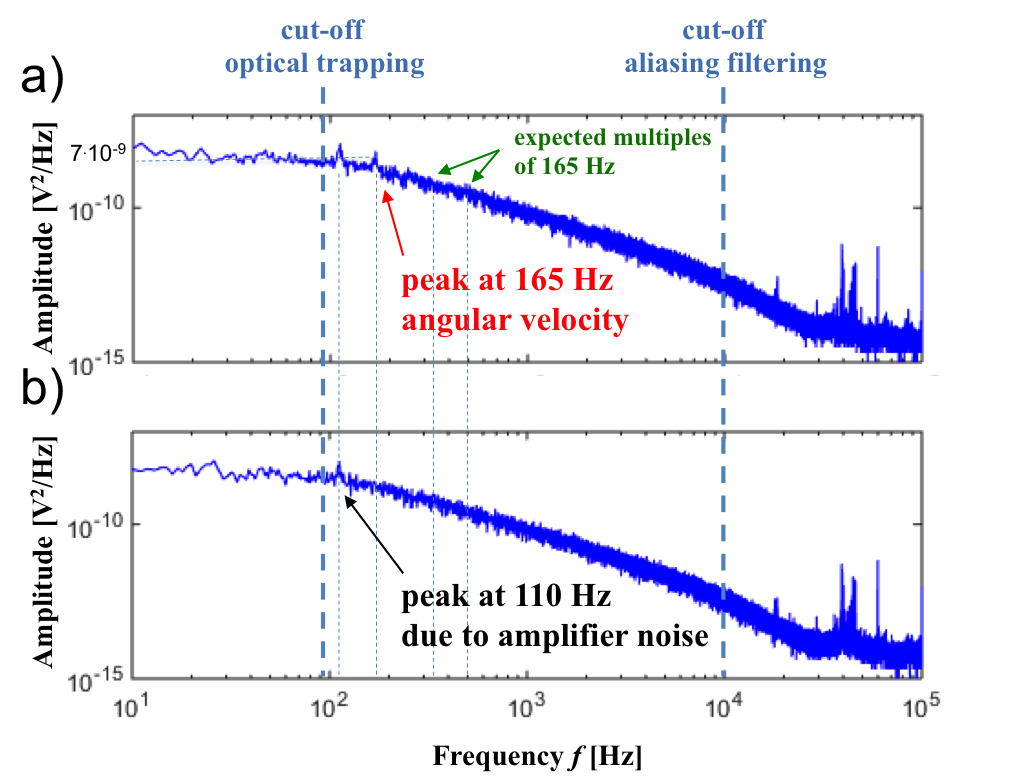
\includegraphics[width=84mm]{Fig9.png}
    \caption{a) Measured power spectrum of an optically trapped 
    \SI{2.06}{\micro\meter} particle that rotated counter-clockwise due to the 
    acoustic VT at \SI{1043}{\kilo\hertz} with \SI{10.0}{\Vrms} and 
    \SI{14.2}{\Vrms} excitation amplitude in $x$- and $y$-direction, 
    respectively. The particle was located at (-0.075, 0.220) \si{\mm}. The 
    spectrum of the $x$-signal (QPD) was recorded and 10 times averaged with a 
    frequency resolution of $\Delta f=\SI{1}{\hertz}$ and a sampling rate of 
    \SI{1}{\MS}. A clear signal peak due to particle rotation at 
  \SI{165}{\hertz} was observed with a signal-to-noise ratio of about 5. The 
signal peak at \SI{110}{\hertz} is related to influences of the acoustic 
excitation set-up.\ b) Control measurement of a non-rotating optically trapped 
\SI{2.06}{\micro\meter} particle under acoustic excitation at 
\SI{1043}{\kilo\hertz} with \SI{1}{\Vrms} and \SI{1.42}{\Vrms} excitation 
amplitude in $x$- and $y$-direction, respectively. A particle rotation was not 
initialized at these low excitation amplitudes and these recorded power spectrum 
of non-rotating \si{\micro\meter} particles were used to identify the peaks not 
related to particle rotation power spectrum due to influences of the environment 
and the acoustic excitation set-up. The peak at \SI{110}{\hertz} is related to 
amplifier noise and vanished when the acoustic excitation set-up was turned off 
\cite{Lamprecht2016}.\label{fig:Fig8}}
\end{figure}
%%%%%%%%%%%%%%%%%%%

%%%%%%%%%%%%%%%%%%%
\begin{figure}[tb]
  \centering
    \begin{tikzpicture}
        \begin{axis}
            [scale only axis,
            width = 69mm,
            height = 5cm,
            xtick = {-0.5,-0.25,0,0.25,0.5},
            xmin = -0.55, xmax = 0.55,
            ymax = 280, ymin = -5,
            xlabel = {Realative x position [\si{\mm}]},
            ylabel = {power spectrum Peak Frequency [\si{\hertz}]}]

            \addplot[red,thick,mark size=4pt,only marks,mark=x] table[x=y, 
            y=f,col sep=comma] {./40_Fitting/datapoints.dat};

            \addplot[thick,blue,dashed] table[x=y, y=f,col sep=comma] 
            {./40_Fitting/datapointsFit.dat};

            \node[blue,above] at (axis cs: 0.16,229) 
            {$\left|229.18\,\sin\left(3.30\,X_{i} + 1.03 \right)\right|$};

        \end{axis}
    \end{tikzpicture}
    \caption{Spatial dependency of frequency peaks (red) due to the acoustic VT 
      from the power spectrum-method. Multiple power spectra of a 
      \SI{2.06}{\micro\meter} silica particle were recorded at specific 
      measurement points in $x$-direction at $x=\SI{0.21}{\mm}\pm\SI{0.5}{\mm}$ 
      and $y=\SI{0.22}{\mm}$. The acoustic field formed two orthogonal standing 
      waves in $x$- and $y$-direction at \SI{1043}{\kilo\hertz} with a relative 
      phase shift of $\zeta =\frac{\pi}{2}$. The determined frequency peaks were 
      fitted to the equation $\left|c_{1}\,\sin(c_2\,X_i + c_3)\right|$ (dashed 
      blue).  The resulting maximal frequency $f$  from the fit was 
      \SI{229}{\hertz} ($ \finalOmega = \SI{13.8e3}{\rpm}$) and the determined 
      acoustic wave in $x$-direction $\lambda_{X}=\sfrac{2\pi}{c_2}$ was 
    \SI{1.90}{\mm}. The pressure nodal point with maximal rotational rate was 
  determined at $x=\SI{0.16}{\mm}$, whereas zero VT was determined at 
$x=\SI{-0.31}{\mm}$ (pressure anti-node).\label{fig:Fig10}}
\end{figure}
%%%%%%%%%%%%%%%%%%%
